\documentclass[12pt,a4paper]{memoir}
% \documentclass[titlepage,12pt,a4paper]{book}

% substituir linha seguinte por 
% \usepackage[english]{babel} 
% se o relatório for escrito na língua inglesa.
\usepackage{siunitx}
\sisetup{math-micro=\text{\textmu},text-micro=$\mu$}
\usepackage[portuguese]{babel}
\usepackage{lipsum}
% \usepackage[utf8]{inputenc}
\usepackage[T1]{fontenc}
\usepackage{fontspec}
\usepackage{textcomp}

\usepackage{makeidx}
\usepackage{xspace}
\usepackage{graphicx,color,times}
\usepackage{fancyhdr}
% \usepackage{pxfonts}
% \usepackage{times}
% \usepackage{mathptm}
% \usepackage{amssymb}
% \usepackage{amsfonts}

\usepackage{amsmath}
\usepackage{latexsym}
\usepackage[printonlyused]{acronym}
\usepackage{float}
\usepackage{listings}
\usepackage{tocbibind}
\usepackage{natbib}
\usepackage{hyperref}
\usepackage{verbatim}
\usepackage{dirtree}

% \usepackage{glossaries}
% \makeglossaries

% \renewcommand{\ttdefault}{phv}

\pagestyle{fancy}
\renewcommand{\chaptermark}[1]{\markboth{#1}{}}
\renewcommand{\sectionmark}[1]{\markright{\thesection\ #1}}
\fancyhf{} \fancyhead[LE,RO]{\bfseries\thepage}
\fancyhead[LO]{\bfseries\rightmark}
\fancyhead[RE]{\bfseries\leftmark}
\renewcommand{\headrulewidth}{0.5pt}
\renewcommand{\footrulewidth}{0pt}
\setlength{\headheight}{15.6pt}
\setlength{\marginparsep}{0cm}
\setlength{\marginparwidth}{0cm}
\setlength{\marginparpush}{0cm}
\addtolength{\hoffset}{-1.0cm}
\addtolength{\oddsidemargin}{\evensidemargin}
\addtolength{\oddsidemargin}{0.5cm}
\addtolength{\evensidemargin}{-0.5cm}


\usepackage{fix-cm}
\usepackage{fourier}
\usepackage[scaled=.92]{helvet}
\definecolor{ChapGrey}{rgb}{0.6,0.6,0.6}
\newcommand{\LargeFont}{
  \usefont{\encodingdefault}{\rmdefault}{b}{n}
  \fontsize{60}{80}\selectfont\color{ChapGrey}
  }
\makeatletter
\makechapterstyle{GreyNum}{
  \renewcommand{\chapnamefont}{\large\sffamily\bfseries\itshape}
  \renewcommand{\chapnumfont}{\LargeFont}
  \renewcommand{\chaptitlefont}{\Huge\sffamily\bfseries\itshape}
  \setlength{\beforechapskip}{0pt}
  \setlength{\midchapskip}{40pt}
  \setlength{\afterchapskip}{60pt}
  \renewcommand\chapterheadstart{\vspace*{\beforechapskip}}
  \renewcommand\printchaptername{
  \begin{tabular}{@{}c@{}}
    \chapnamefont \@chapapp\\}
    \renewcommand\chapternamenum{\noalign{\vskip 2ex}}
    \renewcommand\printchapternum{\chapnumfont\thechapter\par}
    \renewcommand\afterchapternum{
  \end{tabular}
  \par\nobreak\vskip\midchapskip}
  \renewcommand\printchapternonum{}
  \renewcommand\printchaptertitle[1]{
  {\chaptitlefont{##1}\par}}
  \renewcommand\afterchaptertitle{\par\nobreak\vskip \afterchapskip}
}
\makeatother
\chapterstyle{GreyNum}

\setcounter{tocdepth}{3}
\setsecnumdepth{subsubsection}

\renewcommand{\ttdefault}{lmtt}


% NEW COLORS
\definecolor{dark}{gray}{0.25}
\definecolor{lgray}{gray}{0.9}
\definecolor{dkblue}{rgb}{0,0.13,0.4}
\definecolor{dkgreen}{rgb}{0,0.6,0}
\definecolor{gray}{rgb}{0.5,0.5,0.5}
\definecolor{mauve}{rgb}{0.58,0,0.82}

\lstset{ %
  language=C,                    basicstyle=\footnotesize,
  numbers=none,                  numberstyle=\tiny\color{gray}, 
  stepnumber=1,                  numbersep=5pt,
  backgroundcolor=\color{white}, showspaces=false,
  showstringspaces=false,        showtabs=false,
  frame=single,                  rulecolor=\color{black},
  tabsize=2,                     captionpos=b,
  breaklines=true,               breakatwhitespace=false,
  title=\lstname,                keywordstyle=\color{blue},
  commentstyle=\color{dkgreen},  stringstyle=\color{mauve},
  escapeinside={\%*}{*)},        morekeywords={*},
  belowskip=0cm
}

\renewcommand{\lstlistingname}{Excerto de Código}
\renewcommand{\lstlistlistingname}{Lista de Excertos de Código}

\renewcommand{\today}{\day \ifcase \month \or Janeiro\or Fevereiro\or Março\or %
Abril\or Maio\or Junho\or Julho\or Agosto\or Setembro\or Outubro\or Novembro\or %
Dezembro\fi de \number \year} 


\graphicspath{{img/}} %Setting the graphics path

\usepackage{minted}


\begin{document}


\thispagestyle{empty}
\setcounter{page}{-1}

\begin{center}
\begin{Huge}
\textbf{Universidade da Beira Interior}
\end{Huge}
\end{center}

\begin{center}
\begin{Huge}
Departamento de Informática
\end{Huge}
\end{center}

\vspace{0,07cm}
\begin{figure}[!htb]
\centering

\includegraphics[width=191pt]{ubi-fe-di.png}
\end{figure}

\vspace{0.5cm}
\begin{center}
\begin{Large}
\textbf{N\textordmasculine{} 112 - 2019: \emph{Codificação da Cor de Hologramas Digitais Usando Multivistas}}
\end{Large}
\end{center}


\vspace{0.5cm}
\begin{center}
\begin{normalsize}
\begin{large}
Elaborado por:
\end{large}
\end{normalsize}
\end{center}

\vspace{0.2cm}
\begin{center}
\begin{large}
\textbf{Raquel Sofia Brás Guerra}
\end{large}
\end{center}

\vspace{0,5cm}
\begin{center}
\begin{normalsize}
\begin{large}
Orientador:
\end{large}
\end{normalsize}
\end{center}

\vspace{0.2cm}
\begin{center}
\begin{large}
\textbf{Professora Doutora Maria Manuela Areias da Costa Pereira de Sousa}
\end{large}
\end{center}



\vspace{0.5cm}
\begin{center}
\begin{normalsize}
\today
\end{normalsize}
\end{center}


\clearpage{\thispagestyle{empty}\cleardoublepage}

\frontmatter

\chapter*{Agradecimentos}
\label{ch::agradeco_primeiramente_a_deus}




\clearpage{\thispagestyle{empty}\cleardoublepage}


\tableofcontents

\clearpage{\thispagestyle{empty}\cleardoublepage}

\listoffigures

% #   ATENÇÃO
% Se não existirem tabelas, comentar as duas linhas seguintes
\clearpage{\thispagestyle{empty}\cleardoublepage}
\listoftables

% #   ATENÇÃO
% Se existirem trechos de código, descomentar as seguintes linhas
% \clearpage{\thispagestyle{empty}\cleardoublepage}
% \lstlistoflistings

\clearpage{\thispagestyle{empty}\cleardoublepage}
\chapter*{Acrónimos}
\label{ch:acro}

% #   ATENÇÃO
% A lista de acrónimos deve ser ordenada alfanuméricamente.
% Estrangeirismos devem ser realçados em itálico.
% Se o relatório for escrito em Inglês, uma palavra portuguesa é um estrangeirismo.

% O maior acrónimo deve ser colocado neste ponto (reparar que CFIUTE é maior que TCP!).
%               vvvvv
\begin{acronym}[JPEG]
  \acro{ASM}{\textit{Angular Spectrum Method}}
  \acro{JPEG}{\textit{Joint Photographic Experts Group}}
  \acro{kdu}{\textit{Kakadu Software}}
  \acro{PSNR}{\textit{Peak signal-to-noise ratio}}
  \acro{RGB}{\textit{Red, Green \& Blue}}
  \acro{SDK}{\textit{Software Development Kit}}
  \acro{UBI}{Universidade da Beira Interior}
\end{acronym}

% \clearpage{\pagestyle{empty}\cleardoublepage}
% \chapter*{Glossário}
\label{ch::glossario}
\makeglossaries

\newglossaryentry{.NET Framework}
{
  name={.NET Framework},
  description={É uma plataforma para desenvolvimento e funcionamento de aplicações desenvolvida pela Microsoft.}
}

\newglossaryentry{ASP.NET}
{
  name={ASP .Net},
  description={É uma plataforma da Microsoft para o desenvolvimento de aplicações Web e é o sucessor da tecnologia ASP.}
}

\newglossaryentry{CS}
{
  name={C\#},
  description={Lê-se \textit{C Sharp} e é uma linguagem de programação orientada a objectos, desenvolvida pela Microsoft, inicialmente para a plataforma .NET. O C\# é inspirado na junção entre as linguagens C++ e Java.}
}


\newglossaryentry{Java}
{
  name={JAVA},
  description={É uma linguagem de programação orientada a objectos, desenvolvida pela Sun Microsystems na década de 90. Hoje pertence à empresa Oracle.}
}


\newglossaryentry{OpenDMTP}
{
  name={OpenDMTP},
  description={\textit{Open Device Monitoring and Tracking Protocol} é um protocolo e uma \textit{framework} abertos que permite a comunicação bidireccional entre servidores e clientes através da internet.}
}


\newglossaryentry{OpenGTS}
{
  name={Open GTS},
  description={É o primeiro projecto \textit{Open Source} \textit{Web-Based} para controlo de frotas por GPS.}
}


\newglossaryentry{VS2010}
{
  name={Visual Studio 2010},
  description={\textit{Microsoft Visual Studio 2010} é um sistema de desenvolvimento desenvolvido pela Microsoft e é dedicado ao Framework .NET, que contem um conjunto de ferramentas de desenvolvimento projectadas para auxiliar os programadores a enfrentarem desafios complexos.}
}


\newglossaryentry{WebS}
{
	name={Web Service},
	description={Web services são aplicações modulares auto-descritas e auto-contidas, que permitem a integração de sistemas e a comunicação entre aplicações de diferentes tipos.}
}


\newglossaryentry{WebBased}
{
	name={Web Based},
	description={Aplicação desenvolvida para a Web.}
}

\newglossaryentry{Roaming}
{
	name={Roaming},
	description={Define a possibilidade de um utilizador de uma determinada rede obter rede/conecção fora da área geográfica onde foi registado.}
}


\newglossaryentry{Smartphone}
{
	name={Smartphone},
	description={Smartphone é um telefone móvel que contem muitas das principais tecnologias de comunicação e serviços que existem nos computadores pessoais, como acesso a e-mails, serviços de mensagens instantâneas, internet, GPS, entre outros.}
}

\newglossaryentry{TCPIP}
{
	name={TCP/IP},
	description={É um conjunto de protocolos de comunicação entre computadores ligados rede. O nome TCP/IP surge da união entre dois protocolos: o TCP (Transmission Control Protocol) e o protocolo IP (Internet Protocol).}
}

\newglossaryentry{Firewall}
{
	name={Firewall},
	description={É o nome criado para definir um dispositivo para uma rede de computadores que tem como objectivo criar uma política de segurança num determinado ponto de controlo da rede.}
}

\newglossaryentry{JavaScript}
{
	name={JavaScript},
	description={É uma linguagem de programação baseada na linguagem de programação ECMAScript. Actualmente é a linguagem de programação mais utilizada em \textit{``Client-Side''} nos \textit{browsers}.}
}

\newglossaryentry{Flash}
{
	name={Flash},
	description={Desenvolvido pela Macromedia, o Flash é um software utilizado para criação de animações interactivas que funcionam incorporadas em \textit{Browsers}, \textit{Desktop}, \textit{Smartphones}, \textit{Tablets}, e Televisores.}
}


\newglossaryentry{StoredProcedure}
{
	name={Stored Procedure },
	description={É o nome dado a um conjunto de comandos numa base de dados de forma a simplificar a sua utilização.}
}

\newglossaryentry{SQLS}
{
	name={SQL Server 2008},
	description={É um sistema de gestão de base de dados relacional criado pela Microsoft.}
}

\newglossaryentry{Firm}
{
	name={Firmware},
	description={É o conjunto de instruções operacionais programadas directamente no \textit{hardware} de um equipamento electrónico.}
}

\newglossaryentry{browser}
{
	name={Browser},
	description={É um programa de computador que possibilita aos utilizadores uma interacção com documentos virtuais da Internet, também conhecidos como páginas Web.}
}



\clearpage{\thispagestyle{empty}\cleardoublepage}

\mainmatter
\acresetall
\chapter{Introdução}
\label{chap:intro}

\section{Enquadramento}
\label{sec:amb}

A história da captura, armazenamento e visualização de imagens é extremamente rica e milenar. Marcos importantes destacam-se, sendo do particular interesse no Século XXI os grandes passos dados na imagem digital.

Contudo, a vasta maioria da fotografia tem-se centrado na captura de imagens estáticas em duas dimensões. O interesse na captura e representação de objetos e momentos em três dimensões tem ganho um interesse crescente nas últimas décadas.

A área dedicada ao estudo deste modelo, a \textbf{holografia}, carece de vários marcos que já fazem parte do quotidiano da fotografia clássica, nomeadamente padrões \textit{standardizados} para a codificação e compressão de \textbf{hologramas} em formato digital.


\section{Motivação}
\label{sec:mot}
Dada a referida ausência de \textit{standards} no armazenamento e representação da informação, reconstrução e codificação de um holograma, é do interesse da comunidade do JPEG Pleno estudar os codificadores existentes para melhor perceber qual a sua adaptabilidade aos hologramas e quais as modificações necessárias para resolver a falta de padrões nos pontos mencionados.


\section{Objetivos}
\label{sec:obj}
%Neste projeto pretende-se estudar imagens holográficas e o codificador JPEG2000 na codificação de imagens holográficas. Investigar o comportamento do codificador JPEG2000 na codificação da cor quando a codificação é efetuada em diferentes vistas.

Tendo em mente a motivação apresentada na secção \ref{sec:mot}, o presente projeto tem por objetivo principal investigar o desempenho do codec JPEG2000 na codificação de hologramas a cores em multivistas.

Por seu turno, os objetivos secundários --- os quais refletem as diferentes fases da investigação --- são os seguintes:

\begin{enumerate}
  \item Implementar um reconstrutor para hologramas com cor;
  \item Reconstruir hologramas em vários pontos de vista;
  \item Comprimir hologramas reconstruidos com recurso ao codificador JPEG2000;
  \item Avaliar a qualidade das imagens comprimidas face à reconstrução original.
\end{enumerate}

Os objetivos supra-mencionados refletem o objetivo geral de estudar holografia e, assim, expandir o conhecimento na área das tecnologias multimédia.


\section{Organização do Documento}
\label{sec:organ}

\clearpage{\thispagestyle{empty}\cleardoublepage}
\chapter{Estado da Arte}
\label{ch::estado-arte}

\section{Introdução}
\label{sec::estado-arte:intro}

O que é a holografia? O que é um holograma? Como se obtêm, codificam e representam? Que formas já foram estudadas de os comprimir? Como se pode avaliar a qualidade da imagem comprimida?

Estas e outras questões impõem-se perante a investigação que se almeja. A sua resposta, dada no presente Capítulo, orientará a definição de uma estratégia de investigação e permitirá avançar a área da holografia com um renovado conhecimento acerca da compressão de hologramas com a norma JPEG2000.

% ----------------------------------------------------------------------------------------
\section{Perspetiva Histórica e Conceitos Base da Holografia}
\label{sec::estado-arte:hist-base}

% O que é um holograma
Entende-se por \textbf{holograma} uma gravação física de um padrão de interferência que recorre ao efeito de difração da luz para reproduzir um campo de luz tridimensional. Tal resulta numa imagem a qual retém as propriedades da cena original, entre elas a profundidade e a paralaxe\cite{holocenter}.

Por seu turno, a \textbf{holografia} é a ciência envolvida no estudo da obtenção de hologramas.

Há a referir brevemente os seguintes conceitos para clarificação:
\begin{itemize}
  \item \textbf{Difração}: Conjunto de fenómenos que ocorrem quando uma onda encontra um obstáculo, em particular a sua aparente flexão e alargamento ao atravessar orifícios\cite{Grimaldi2010,Cajori1929};
  \item \textbf{Interferência}: Semelhante à difração, mas referente à sobreposição de duas ou mais ondas;
  \item \textbf{Paralaxe}: Diferença na posição aparente de um objeto quando observado em locais diferentes\cite{stevenson2007shorter,waite2013pocket}.
\end{itemize}


\begin{figure}[!htbp]
  \centering
  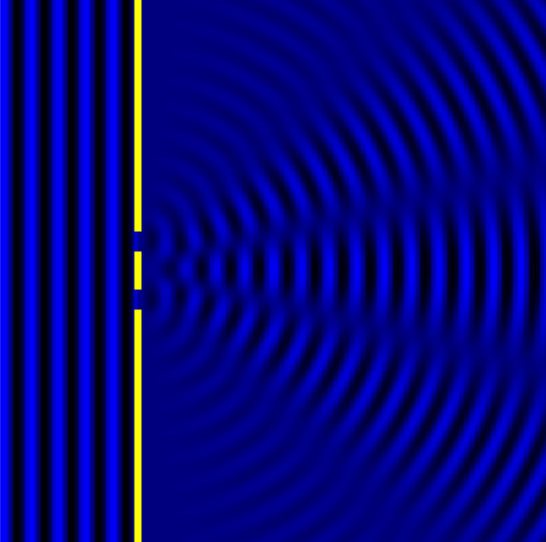
\includegraphics[width=0.5\textwidth]{Doubleslit}
  \caption[Ilustração do efeito de difração.]{Ilustração do efeito de difração de uma onda a atravessar dois orifícios vizinhos\cite{img:doubleslit}.}
  \label{fig:diffraction}
\end{figure}

\begin{figure}[!htbp]
  \centering
  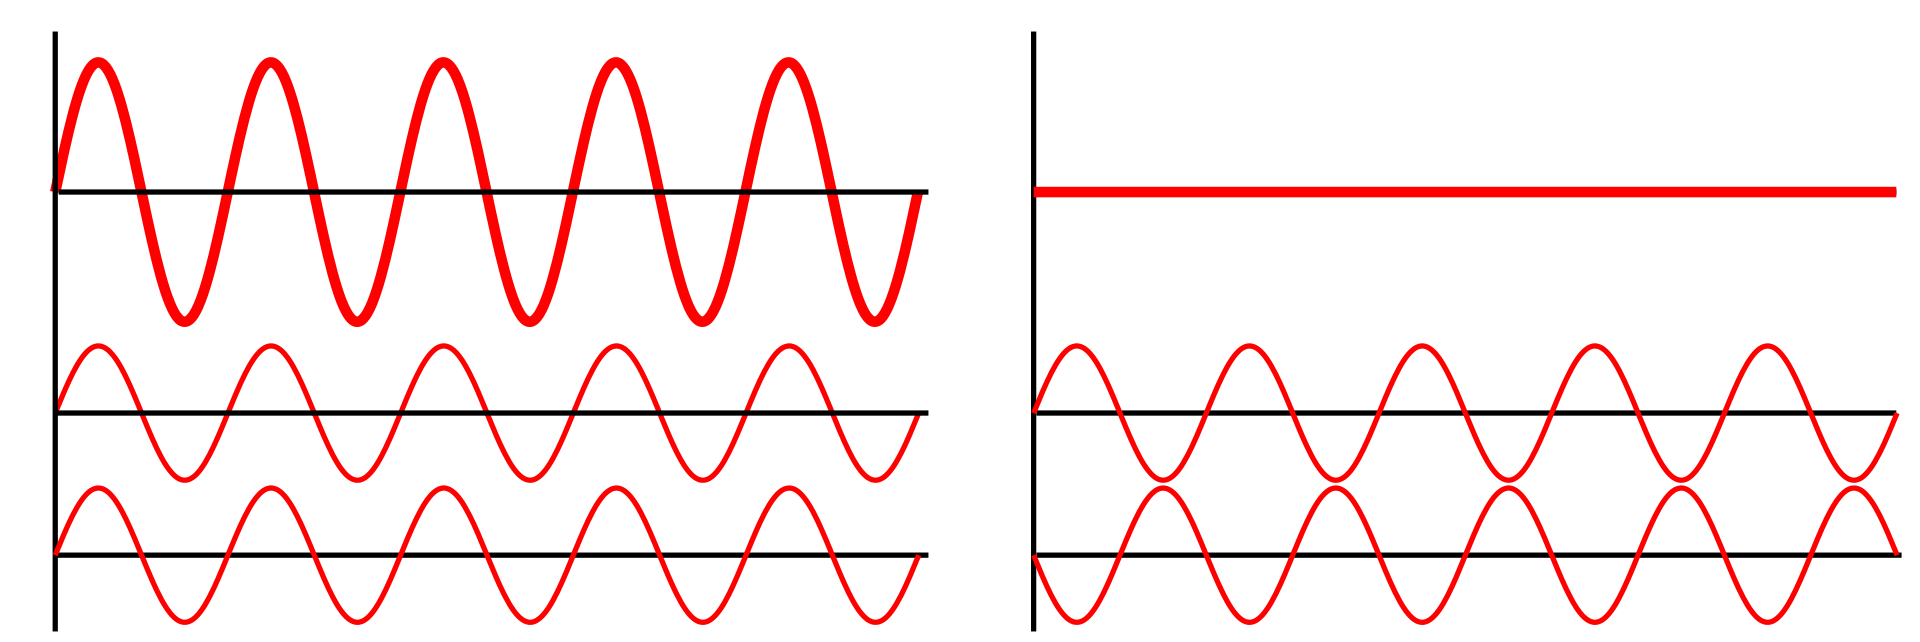
\includegraphics[width=\textwidth]{Interference}
  \caption[Ilustração do efeito de interferência.]{Ilustração do efeito de interferência de duas ondas\cite{img:interference}. Do lado esquerdo encontra-se representada uma interferência construtiva: as duas ondas sincronizadas (\textit{i.e.} exatamente em fase) produzem uma nova onda de amplitude aumentada. Do lado direito apresenta-se um caso de interferência destrutiva: existe uma anulação das ondas por estarem exatamente fora de fase.}
  \label{fig:interference}
\end{figure}

\begin{figure}[!htbp]
  \centering
  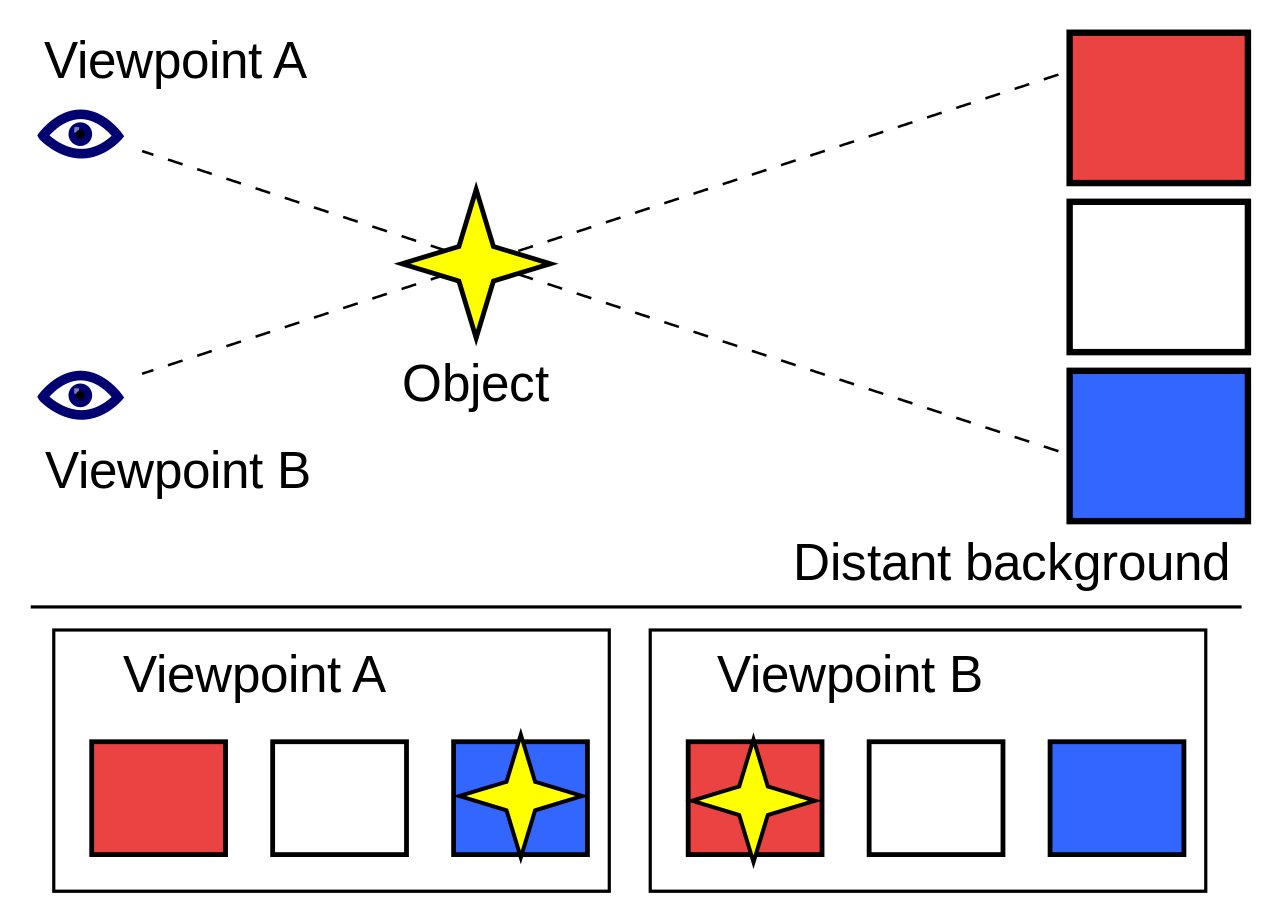
\includegraphics[width=0.6\textwidth]{parallax}
  \caption[Ilustração do efeito de paralaxe.]{Ilustração do efeito de paralaxe de um objeto face a um padrão de fundo\cite{img:parallax}. Devido à mudança de perspetiva do utilizador em dois pontos de vista distintos, no ponto A o observador perceciona a estrela como estando sobre o fundo azul, enquanto no ponto B esta aparenta estar sobre o fundo vermelho.}
  \label{fig:parallax}
\end{figure}


Enquanto a fotografia tradicional apenas captura a intensidade da luz refletida pelos objetos, a holografia permite capturar tanto a amplitude como a fase da onda de luz dispersa por um objeto\cite{holocenter,Image2018,spencer1973the}.

Em contraste face à fotografia clássica, a qual teve as suas origens desde a descoberta da \textit{camara obscura} por parte da China Antiga\cite{Krebs2004}, a holografia como ciência conheceu o seu início com o cientista húngaro-britânico Dennis Gabor na década de 1940 enquanto este estudava avanços na tecnologia da microscopia eletrónica\cite{GABOR1948, GABOR1949}. A descoberta da holografia e, por sua vez, dos hologramas foi inesperada.

A técnica foi adaptada e é ainda hoje utilizada na microscopia eletrónica no que se chama de \textbf{holografia eletrónica}. Contudo, a \textbf{holografia ótica} só pôde avançar após a invenção do \textit{laser} na década de 1960\cite{Leith1962,Leith1964}.

O ponto-chave no desenvolvimento de imagens holográficas, proposto por Dennis Gabor em 1948 numa tentativa de melhorar a microscopia eletrónica, é o uso de uma fonte de luz de referência para codificar uma onda sobreposta com outra a fim de registar os padrões de interferência\cite{GABOR1948}. Contudo, as experiências de Gabor eram limitadas pelo uso de ondas óticas paralelas ao eixo ótico\cite{Image2018}.

Desta forma, em 1962, Emmet Leith e Juris Upatnieks desenvolveram a técnica que viria a lançar em definitivo a holografia ótica: a \textbf{holografia ótica \textit{off-axis}}\cite{Leith1962}, ou seja, o eixo ótico não é paralelo ao feixe de ondas óticas. Esta técnica, desenvolvida no âmbito do estudo de radares, teve a sua prova prática após a invenção do \textit{laser} e, em 1964, os dois cientistas produziram uma série de hologramas que culminariam na atribuição do Prémio Nóbel da Física a Dennis Gabor em 1971\cite{Leith1962,nobel1971}.

Diferentes tipos de hologramas óticos foram desenvolvidos nas décadas subsequentes, assim como outras áreas beneficiaram com os estudos enveredados na área da holografia\cite{Image2018}. Em particular, o desenvolvimento de hologramas visualizados pela transmissão de luz branca, por Stephen Benton\cite{benton1977}, permitiu avanços na medicina, em particular na área da imagiologia, onde a holografia foi incorporada em exames como a \ac{TAC} e a \ac{RMN}\cite{Saxon2003}. Curiosamente, esta técnica é comummente vista em cartões de crédito/débito e documentos de identificação nacional oficiais\cite{Saxon2003,Toal2012}.




\section{O Holograma}
\label{sec::estado-arte:holograma}

Existem atualmente duas formas de obter e reconstruír hologramas\cite{Image2018}:
\begin{enumerate}
  \item Configuração \textbf{analógica} (método original);
  \item Configurações \textbf{digitais}.
\end{enumerate}

De notar que existem diferentes métodos tanto para a obtenção como para a reconstrução numérica na holografia digital (Figura \ref{fig:holografia}).

A \textbf{holografia digital} em particular é um processo de três passos\cite{Image2018}:
\begin{enumerate}
  \item Geração do campo de ondas do objeto;
  \item Aquisição (ou registo) do padrão de interferência;
  \item Reconstrução do campo do objeto para visualização tridimensional ou em multivista bidimensional renderizada.
\end{enumerate}

As configurações digitais serão as abordadas na presente Secção, sendo a analógica ignorada, uma vez que ambas apresentam princípios teóricos semelhantes e o âmbito do projeto é a holografia digital. Em particular, serão abordadas apenas as técnicas utilizadas na obtenção e reconstrução dos hologramas testados no projeto.


\subsection{Obtenção}
\label{ssec::estado-arte:holograma:obter}

A obtenção de um holograma envolve a codificação da amplitude e da fase da onda de luz dispersa por um objeto. Esta varia conforme o meio onde o holograma será gravado. Uma vez que os métodos clássicos são tendencialmente dispendiosos e morosos, a atenção maior da comunidade científica tem sido no desenvolvimento de métodos digitais\cite{Image2018}.

Em particular, um \textbf{\ac{HGC}} envolve um processo no qual o campo de ondas do objeto é computado digitalmente através de uma simulação da propagação da luz dispersa pela cena face ao plano do holograma.

De entre os métodos de \textbf{obtenção indireta} {\textit{i.e.} geração de hologramas por computador}, sumariados na Figura \ref{fig:holografia}, dois em particular serão resumidos por serem os utilizados para a obtenção dos hologramas objeto de teste no projeto\cite{holorepo2018,Gilles2016}:

\begin{enumerate}
  \item \textit{Point-source}\cite{Image2018,Brown1966}:\\
    É feita uma amostragem à cena tridimensional através da recolha de pontos considerados como fontes esféricas de luz. Contudo, esta técnica é de uma grande complexidade computacional (ordem $O(NM)$, onde $N$ representa o número de pixeis do holograma e $M$ é o número total de pontos da cena).

  \item \textit{Layer-based}\cite{Image2018,Lohmann1978} (também conhecido por \textit{wave-field}\cite{Gilles2016}):\\
    A cena tridimensional é dividida em camadas paralelas ao plano do holograma. Cada camada é considerada uma fonte superficial de luz cujas emissões de ondas luminosas são propagadas numericamente para o plano do holograma e somadas para obter o campo de ondas do objeto. Esta técnica apresenta uma complexidade computacional inferior face ao \textit{point-source} (nomeadamente $O(N_z N \log (N))$, onde $N$ representa o número de pixeis do holograma e $N_z$ é o número de camadas). Todavia, esta técnica não é aconselhável para cenas de grande profundidade.
\end{enumerate}

\begin{figure}[!htbp]
  \centering
  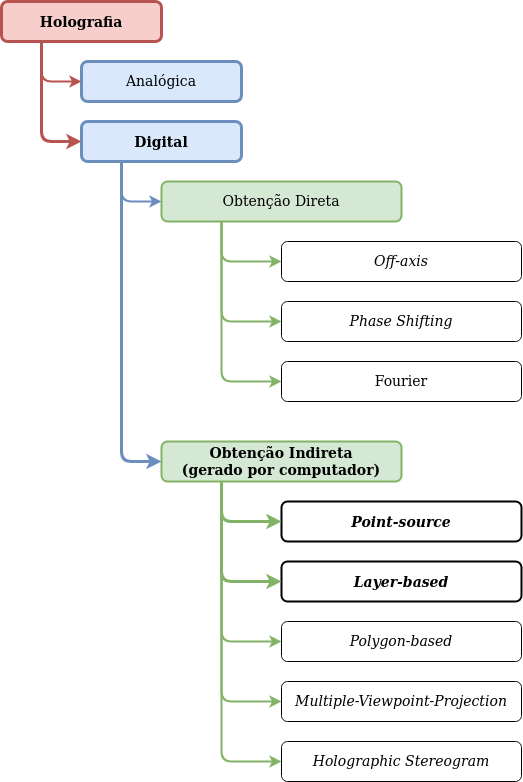
\includegraphics[width=.9\textwidth]{holografia}
  \caption[Métodos de obtenção de hologramas.]{Métodos de obtenção de hologramas\cite{Image2018}. A negrito estão destacados os métodos utilizados na obtenção dos hologramas testados no presente projeto.}
  \label{fig:holografia}
\end{figure}

\begin{figure}[!htbp]
  \centering
  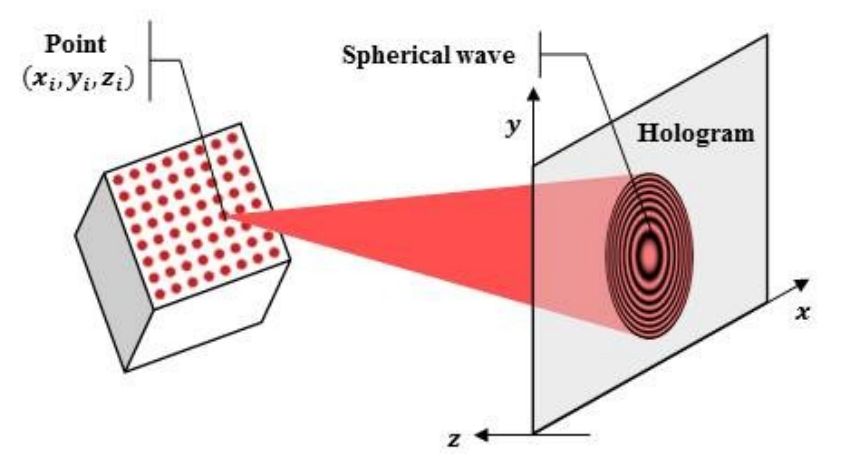
\includegraphics[width=.9\textwidth]{point-source}
  \caption[Obtenção de um \acs{HGC} pela técnica \textit{point-source}]{Obtenção de um \acs{HGC} pela técnica \textit{point-source}\cite{Image2018}.}
  \label{fig:point-source}
\end{figure}

\begin{figure}[!htbp]
  \centering
  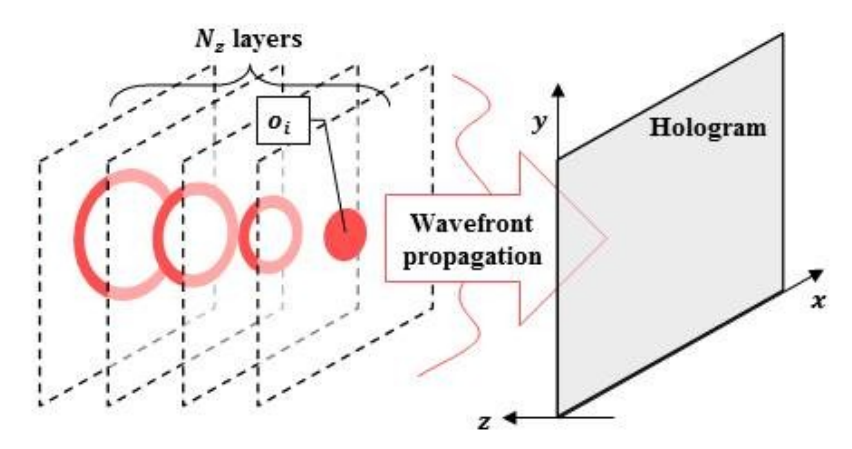
\includegraphics[width=.9\textwidth]{layer-based}
  \caption[Obtenção de um \acs{HGC} pela técnica \textit{layer-based}]{Obtenção de um \acs{HGC} pela técnica \textit{layer-based}\cite{Image2018}.}
  \label{fig:layer-based}
\end{figure}


\subsection{Reconstrução}
\label{ssec::estado-arte:holograma:reconst}

Esta fase do processo da holografia digital pode ser alcançada de duas formas\cite{Image2018}:
\begin{enumerate}
  \item \textbf{Reconstrução numérica}, onde é feita simulação da difração da luz por parte do holograma digitalmente obtido;
  \item \textbf{Reconstrução ótica}, com a propagação física de um feixe ótico com recurso a um \textit{laser} e a um \ac{SLM}.
\end{enumerate}

Apenas o primeiro tipo de reconstrução será abordado por ser o utilizado no projeto.

São então definidos três métodos de reconstrução numérica consoante a distância de reconstrução\cite{Image2018}:
\begin{enumerate}
  \item \ac{ASM} (curta distância);
  \item \ac{HCM} (média-longa distância);
  \item \ac{FTM} (longa distância).
\end{enumerate}

O que será utilizado no projeto é o método \textbf{\ac{ASM}}. Não sendo objetivo máximo deste Capítulo explanar em detalhe os conceitos teóricos inerentes a este método, segue-se um breve resumo para esclarecimento com as principais fórmulas que serão diretamente utilizadas no desenvolvimento de \textit{scripts} no âmbito da investigação.

% \subsubsection{\acf{ASM}}
% \label{sssec::estado-arte:holograma:reconst:asm}

A \textbf{reconstrução numérica} de um holograma consiste na propagação da amplitude complexa registada do objeto no plano da câmara digital relativa à sua posição original. Esta é feita com recurso à teoria de difração escalar (Figura \ref{fig:diffraction-theory})\cite{Image2018}, a qual estabelece que um campo difratado $\psi_p(x,y;z)$ pode ser obtido a partir do campo incidente $\psi_{p_0}(x,y)$ de acordo com a equação (\ref{eq:diffracted-field})\cite{Poon2014},

\begin{equation}
  \psi_p(x,y;z) = \mathcal{F}^{-1}\left\{\mathcal{F}\left\{\psi_{p_0}(x,y)\right\}\times\mathcal{H}(k_x,k_y;z)\right\}
  \label{eq:diffracted-field}
\end{equation}

onde $\mathcal{H}(k_x,k_y;z)$ é a \ac{SFTF} (equação (\ref{eq:stft})).

\begin{figure}[!bp]
  \centering
  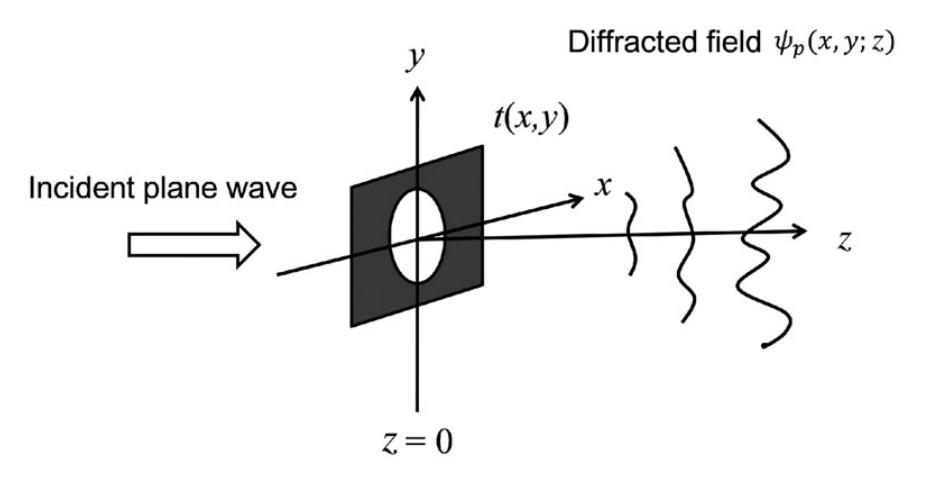
\includegraphics[width=.9\textwidth]{diffraction-theory}
  \caption[Geometria da difração.]{Geometria da difração, onde $t(x,y)$ é um ecrã de difração\cite{Poon2014}.}
  \label{fig:diffraction-theory}
\end{figure}

\begin{equation}
  \mathcal{H}(k_x,k_y;z) = \exp\left[2j\pi z\sqrt{\frac{1}{\lambda^2}-k_x^2-k_y^2}\right]
  \label{eq:stft}
\end{equation}

De notar que:
\begin{itemize}
  \item $\lambda$ é o comprimento de onda do feixe de luz;
  \item $\mathcal{F}$ é a Transformada de Fourier;
  \item $k_x$ e $k_y$ são as frequências espaciais radianas.
\end{itemize}

A equação (\ref{eq:diffracted-field}) é a fórmula de base do método \ac{ASM} (também conhecido por Método da Dupla Transformada de Fourier ou Método de Convolução)\cite{Poon2014}.


\subsection{Representação}
\label{ssec::estado-arte:holograma:rep}

Os dados holográficos podem ser representados de várias formas. Embora sejam todas equivalentes no sentido em que representam o mesmo objeto, algumas tornam a compressão mais eficiente. 

No âmbito deste projeto, apenas é relevante a representação no campo de onda complexo, o qual pode englobar\cite{Image2018}:

\begin{itemize}
    \item \textbf{Dados reais e imaginários}: utilizam um sistema de coordenadas cartesiano para representar amplitudes complexas;
    \item \textbf{Dados da amplitude e fase}: os valores complexos são expressos num sistema de coordenadas polares.
\end{itemize}

Os hologramas utilizados neste projeto são representados pelo formato de \textbf{amplitude-fase} (Figura \ref{fig:ampli-fase}).


\begin{figure}[!htbp]
  \centering
  \begin{tabular}{c c}
    \includegraphics[width=0.4\textwidth]{piano4k_ampli} &
    \includegraphics[width=0.4\textwidth]{piano4k_phase} \\
     Amplitude & Fase \\
  \end{tabular}
  \caption[Exemplo de um holograma no formato amplitude-fase]{Exemplo do holograma \texttt{piano4k} no formato amplitude-fase.}
  \label{fig:ampli-fase}
\end{figure}


\section{Compressão de um Holograma}
\label{sec::estado-arte:compress}


Dado que a dimensão dos ficheiros digitais pode ser avultada, tem sido do interesse da área da holografia estudar métodos eficientes de compressão que não comprometam a qualidade dos hologramas.

Neste sentido, o primeiro modelo de codificação e transmissão digital de hologramas foi proposto em 1991. Este envolvia a modulação dos dados num sinal de televisão com recurso a uma versão modificada do MPEG-2\cite{Sato1991}. 
Em 1993, o recurso aos formatos MPEG-1 e MPEG-2 foi novamente proposto para a compressão de segmentos do holograma correspondentes a diferentes perspetivas de reconstrução\cite{YOSHIKAWA1993,Yoshikawa1996}.

Contudo, apenas em 2002 foi concluído que os melhores rácios de compressão são esperados quando os hologramas digitais são representados pelas suas componentes real e imaginária de forma independente\cite{Naughton2002}.

Desde então vários estudos têm sido feitos no sentido de perceber os melhores métodos de compressão, incluindo estudos baseados na quantização escalar\cite{Arrifano}
e formatos com perda (\textit{e.g.} JPEG, JPEG2000, MPEG-4 AVC, Dirac e HEVC)\cite{Xing2014,Darakis2010,Peixeiro2016,Pinheiro2018}.

Sendo o formato JPEG2000 o investigado no presente projeto, este será seguidamente abordado.


\subsection{Uma Breve Introdução ao JPEG2000}
\label{ssec::estado-arte:compress:jpeg2000}

O formato JPEG2000 é uma norma internacional para a compressão de imagens. Esta foi elaborada com o objetivo de mitigar os problemas e as limitações enfrentadas com o formato \ac{JPEG} clássico de 1992. Uma das abordagens para alcançar este objetivo foi a substituição do uso de \ac{DCT} para um método baseado na transformada \textit{wavelet}\cite{Taubman2002}.

Conforme verificado pela Parte 1 da norma JPEG2000, algumas das vantagens a destacar são\cite{Pierre-AnthonyLemieux,Taubman2002}:
\begin{itemize}
  \item \textit{Eficiência de compressão}:\\ Em média \SI{20}{\percent} superior face ao \ac{JPEG} clássico.
  \item \textit{Escalabilidade da qualidade}:\\ Possibilidade de extrair praticamente qualquer qualidade reduzida.
  \item \textit{Escalabilidade da resolução}:\\ Possibilidade de extrair qualquer resolução que seja relacionada a uma potência de 2.
  \item \emph{Acessibilidade da \ac{ROI}}:\\ Habilidade de reconstruir uma região espacial arbitrária.
  \item \textit{Paralelismo}:\\ Capacidade de utilizar computação paralela com recurso a:
  \begin{itemize}
    \item Múltiplos \textit{cores} de uma \ac{CPU};
    \item Várias \textit{threads} numa \ac{GPU};
    \item \textit{Hardware} dedicado.
  \end{itemize}
  \item \textit{Controlo ótimo não-iterativo do rácio}:\\ Poder de alcançar um tamanho de compressão alvo sem recorrer a codificação iterativa.
\end{itemize}
% ISO/IEC JTC 1/SC 29/WG1 | Document N87018

Contudo, a norma JPEG2000 enfrenta como principal desvantagem o facto de ser computacionalmente bastante mais exigente, em especial com conteúdo de muito alta qualidade (\ac{UHD}).

A compressão nesta norma envolve várias fases, a saber\cite{Taubman2002a}:
\begin{enumerate}
  \item \textit{Transformada de cor}:\\ As imagens no formato \ac{RGB} são inicialmente transformadas num novo espaço de cor, havendo duas possibilidades para tal:
  \begin{enumerate}
    \item \acf{ICT}:\\ Transforma para o modelo YCbCr com recurso a números de vírgula flutuante ou de ponto fixo que geram erros de arredondamento (sendo assim chamado de ``irreversível'').
    \item \acf{RCT}:\\ Transforma para um modelo YUV modificado que não introduz erros de quantização (sendo, portanto, ``reversível''). As transformações são:\\
    \begin{tabular}{r @ {~=~} l @{~~;~~~~~} r @ {~=~}  l @{~;}}
      $Y$   & $\left\lfloor\frac{R+2G+B}{4}\right\rfloor$ & $G$ & $Y-\left\lfloor\frac{C_B+C_R}{4}\right\rfloor$ \\
      $C_B$ & $B-G$ & $R$ & $C_R+G$ \\
      $C_R$ & $R-G$ & $B$ & \multicolumn{1}{l @{~.}}{\hspace{-6pt}$C_B+G$} \\
    \end{tabular}
  \end{enumerate}
  
  \item Tiling:\\ A imagem é dividida em \textit{tiles}, \textit{i.e.} regiões retangulares que são codificadas separadamente. Cada \textit{tile} pode ter um tamanho qualquer, podendo a imagem completa ser, no limite, uma \textit{tile}. Todas as \textit{tiles} têm o mesmo tamanho. Esta fase pode introduzir o mesmo efeito de blocos encontrado na norma \ac{JPEG} clássica e pode ainda condicionar o valor de \ac{PSNR} da imagem comprimida.
  
  \item \textit{Transformada \emph{wavelet}}:\\ Cada \textit{tile} passa por uma transformada \textit{wavelet} de tamanho arbitrário (\textit{versus} o tamanho padrão de $8 \times 8$ do \ac{JPEG} clássico). Semelhante à transformada de cor, existem dois tipos de transformada \textit{wavelet}:
  \begin{enumerate}
    \item \textit{Irreversível}:\\ Introduz ruído de quantização.
    \item \textit{Reversível}:\\ Recorre exclusivamente a coeficientes inteiros, pelo que não é necessário arredondamento, prevenindo assim a inserção de ruído de quantização\cite{Bovik2009,LeGall,Unser2003}.
  \end{enumerate}
  
  \item \textit{Quantização}:\\ Os coeficientes passam por uma quantização escalar a fim de reduzir o número de \textit{bits} para os representar. O passo de quantização permite controlar a taxa de compressão: um maior passo de quantização aumenta a compressão, mas com a desvantagem natural de diminuir a qualidade final. Um passo de quantização unitário (\textit{i.e.} com valor $1$) leva a que este passo não seja sequer realizado.
  
  \item \textit{Codificação}:\\ Passo complexo que envolve um processo denominado \ac{EBCOT}. Os detalhes deste passo ultrapassam o âmbito do projeto.
\end{enumerate}

Os ficheiros resultantes têm tradicionalmente a extensão \verb|*.jp2|. Há ainda a referir o formato \verb|*.jpx| com o qual se podem incluir animações.

Por fim, os metadados de uma imagem codificada com a norma JPEG2000 são armazenados no formato \ac{XML}\cite{bib:jpeg2000}, contrastando com o formato tradicional \textit{Exif} utilizado pela norma \ac{JPEG} clássica e outras normas de compressão e armazenamento de multimédia.


\subsection{\acs{PSNR}: uma Métrica de Relação Qualidade-Débito}
\label{ssec::estado-arte:compress:psnr}

\textbf{\acf{PSNR}} é uma métrica utilizada na área da engenharia que calcula o rácio entre a potência máxima possível de um sinal e a potência de sinais de ruído que afetam a fiabilidade da sua representação. Esta é expressa em \acf{dB}. A fórmula do \ac{PSNR} é dada pela equação (\ref{eq:psnr})\cite{salomon2007data},

\begin{equation}
  \mathrm{PSNR} = 20\cdot\log\left(\mathrm{MAX}_I\right) - 10\cdot\log\left(\mathrm{MSE}\right)
  \label{eq:psnr}
\end{equation}

onde:
\begin{itemize}
  \item $\mathrm{MAX}_I$ é o valor máximo possível do píxel da imagem (para uma representação com $n$ \textit{bits}, o valor será dado por $2^n-1$);
  \item \ac{MSE} (\textit{i.e.} erro médio quadrado) é dado pela equação (\ref{eq:psnr-mse}):
    \begin{equation}
      \mathrm{MSE} = \frac{1}{mn}\sum_{i=0}^{m-1}\sum_{j=0}^{n-1}\left[I(i,j)-K(i,j)\right]^2
      \label{eq:psnr-mse}
    \end{equation}
\end{itemize}

Para multimédia codificada com 8 \textit{bits} de profundidade em formatos com perdas, o valor de \ac{PSNR} ronda tipicamente os \SI{30}{\decibel} a \SI{50}{\decibel}\cite{welstead1999fractal,barni2006document}.


\section{Conclusões}
\label{sec::estado-arte:conclusao}
Apesar da holografia ser uma área com décadas de história e pesquisa, esta ainda carece de normas bem estabelecidas a fim de tornar a sua manipulação, o seu estudo e o seu uso exequíveis de uma forma prática.

Assim, com base no conhecimento de interesse coletado acerca da holografia e da compressão de imagens, torna-se necessário definir quais os materiais, as ferramentas e as tecnologias necessárias para a concretização da investigação nesta área.

\clearpage{\thispagestyle{empty}\cleardoublepage}
\chapter{Tecnologias e Ferramentas Utilizadas}
\label{ch::tecno-ferr}

\section{Introdução}
\label{sec::tecno-ferr:intro}

O projeto apresentado só foi possível ser concluído devido à existência de tecnologias e ferramentas, assim como de materiais, os quais se revelaram essenciais.

Em particular, este Capítulo aborda:

\begin{itemize}
    \item O \textit{software} de reconstrução de hologramas;
    \item A escolha da linguagem de programação para o projeto;
    \item O \ac{SDK} de codificação de imagens no formato JPEG2000;
    \item O \textit{hardware} utilizado;
    \item Os hologramas testados.
\end{itemize}

% Cada capítulo \underline{intermédio} deve começar com uma breve introdução onde é explicado com um pouco mais de detalhe qual é o tema deste capítulo, e como é que se encontra organizado (i.e., o que é que cada secção seguinte discute).


\section{Tecnologias e Ferramentas}
\label{sec::tecno-ferr:tecno-ferr}

O desenvolvimento do projeto envolveu o trabalho conjunto de diversas ferramentas, nomeadamente Python 3, \textit{Kakadu Software} e \textit{software} escrito no âmbito do projeto JPEG Pleno.

\subsection{Software de Reconstrução de Hologramas e sua Transcrição para Python}

Do 80\textordmasculine~Encontro do Grupo JPEG, realizado em Berlim entre 7 e 13 de julho de 2018, resultou um software desenvolvido por Antonin Gilles e Patrick Gioia, do \textit{Institute of Research \& Technology b<>com}. O respetivo código, fornecido pela professora orientadora, encontra-se implementado em MATLAB.

Dada a ausência de uma licença do MATLAB para utilizar este \textit{sofware} desenvolvido no âmbito do JPEG Pleno, foi necessário transcrever o código para uma nova linguagem de programação. Neste sentido, optou-se pelo Python 3.

% Sendo uma linguagem , de utilização gratuita e com a vantagem de ser mais eficiente face ao MATLAB, 

O recurso a Python apresenta uma miríade de vantagens, entre elas:
\begin{itemize}
    \item Linguagem \textit{open source};
    \item Utilização e distribuição gratuita da linguagem;
    \item Maior eficiência face ao MATLAB;
    \item Utilização comum no contexto de processamento multimédia e respetivos projetos;
    \item Vasto leque de bibliotecas, facilitando a implementação de \textit{software} específico;
    \item Abundância de documentação;
    \item Forte comunidade \textit{online} de suporte.
\end{itemize}

A escolha do Python foi, portanto, natural no âmbito do presente projeto.

Durante a fase de transcrição decorreu uma atualização do Python, tendo sido a última versão do código executada e testada na versão 3.8.2 em três distribuições GNU/Linux de 64 bits: Ubuntu 18.04 LTS, Fedora 31 e Linux Mint 20.

\subsection{\textit{Kakadu Software}}
\label{ssec::tecno-ferr:tecno-ferr:kdu}
Uma vez que o JPEG2000 é o formato alvo deste projeto, e tendo em conta a dificuldade encontrada em projetos anteriores no contexto da holografia em utilizar a ferramenta \textit{FFmpeg}, foi recomendado pela professora orientadora a utilização do \textit{Kakadu Software}.

Este é um \ac{SDK} para codificação e descodificação de imagens com recurso ao formato JPEG2000, segundo o \textit{standard} pela \ac{JPEG}.

Os comandos deste \ac{SDK} de relevo para o projeto são os seguintes:

\begin{enumerate}
    \item \texttt{kdu\_compress}: codifica uma imagem para o formato JPEG2000.\\
    Sintaxe:
    \begin{minted}[breaklines,frame=lines]{bash}
kdu_compress -i input_file -o output_file -rate n Cycc=<yes|no> -precise -quiet
    \end{minted}
    onde:
    \begin{itemize}
        \item \verb|-i input_file|: imagem de \textit{input};
        \item \verb|-o output_file|: ficheiro de \textit{output};
        \item \verb|-rate n|: número de \textit{bits} por amostra ($n$ pode ser um número flutuante);
        \item \verb#Cycc=<yes|no>#: \verb|yes| caso seja usada a codificação com transformada de cor de \ac{RGB} para YCbCr, \verb|no| em caso contrário;
        \item \verb|-precise|: força o uso de representações de 32 \textit{bits};
        \item \verb|-quiet|: suprime o \textit{output} do programa.
    \end{itemize}
    
    \item \texttt{kdu\_expand}: descodifica uma imagem no formato JPEG2000.\\
    Sintaxe:
    \begin{minted}[breaklines,frame=lines]{bash}
kdu_expand -i input_file -o output_file -rate n -quiet
    \end{minted}
    onde:
    \begin{itemize}
        \item \verb|-i input_file|: imagem de \textit{input};
        \item \verb|-o output_file|: ficheiro de \textit{output};
        \item \verb|-rate n|: número de \textit{bits} por amostra ($n$ pode ser um número flutuante);
        \item \verb|-quiet|: suprime o \textit{output} do programa.
    \end{itemize}
\end{enumerate}

% 'kdu_compress -i {} -o {} -rate {} Cycc={} -precise -quiet'
% 'kdu_expand -i {} -o {} -rate {} -precise -quiet'

\section{Materiais Utilizados}
\label{sec::tecno-ferr:materiais}

\subsection{\textit{Hardware}}
\label{ssec::tecno-ferr:materiais:hardware}

De notar que esta implementação do \textit{software} de reconstrução de hologramas requer computadores com especificações mais generosas.

Para este projeto, dois computadores em particular executaram as várias iterações de desenvolvimento do \textit{software} transcrito em Python:
\begin{enumerate}
    \item \textit{Desktop}: processador Ryzen\texttrademark~7 2700X \@ 3.7--4.3GHz, placa gráfica NVidia\textsuperscript{\textregistered} Quadro K5000 (4GB), memória RAM de 32GB e \textit{swap} de 96GB, armazenamento SSD de 1TB;
    \item Portátil: Intel\textsuperscript{\textregistered}~Core\texttrademark~i5-10210U \@ 1.6--4.2GHz, memória RAM de 16GB e \textit{swap} de 8GB, armazenamento SSD de 512GB.
\end{enumerate}

\subsection{Hologramas}
\label{ssec::tecno-ferr:materiais:hologramas}

Os hologramas reconstruidos com o \textit{software} desenvolvido no âmbito deste projeto são fornecidos pelo \textit{Institute of Research \& Technology b<>com}. De entre os disponíveis, foram utilizados os seguintes hologramas com as respetivas características:
\begin{enumerate}
    \item \texttt{Dices4k} (Figura \ref{fig:bcom_dices4k}):
          \begin{itemize}
              \item Resolução: 4096$\times$4096;
              \item \textit{Pixel pitch}: \SI{0.4}{\micro\meter};
              \item Comprimento de onda vermelho: \SI{640}{\nano\meter};
              \item Comprimento de onda verde: \SI{532}{\nano\meter};
              \item Comprimento de onda azul: \SI{473}{\nano\meter};
              \item Localização da cena: entre \SI{0.164}{} e \SI{0.328}{\centi\meter}.
          \end{itemize}
    \item \texttt{DiffuseCar4k} (Figura \ref{fig:bcom_diffuseCar4k}):
          \begin{itemize}
              \item Resolução: 4096$\times$4096
              \item \textit{Pixel pitch}: \SI{0.4}{\micro\meter};
              \item Comprimento de onda vermelho: \SI{640}{\nano\meter};
              \item Comprimento de onda verde: \SI{532}{\nano\meter};
              \item Comprimento de onda azul: \SI{473}{\nano\meter};
              \item Localização da cena: entre \SI{0.11}{} e \SI{0.25}{\centi\meter}.
          \end{itemize}
    \item \texttt{Piano4k} (Figura \ref{fig:bcom_piano4k}):
          \begin{itemize}
              \item Resolução: 4096$\times$4096
              \item \textit{Pixel pitch}: \SI{0.4}{\micro\meter};
              \item Comprimento de onda vermelho: \SI{640}{\nano\meter};
              \item Comprimento de onda verde: \SI{532}{\nano\meter};
              \item Comprimento de onda azul: \SI{473}{\nano\meter};
              \item Localização da cena: entre \SI{0.17}{} and \SI{0.313}{\centi\meter}.
          \end{itemize}
\end{enumerate}

\begin{figure}
    \centering
    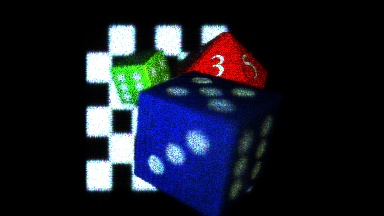
\includegraphics[width=\textwidth]{bcom_dices4k.jpg}
    \caption{Holograma \texttt{Dices4k} (imagem original).}
    \label{fig:bcom_dices4k}
\end{figure}

\begin{figure}
    \centering
    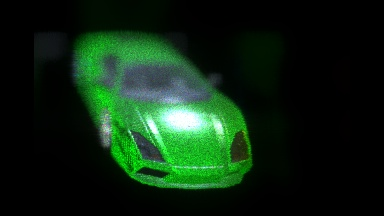
\includegraphics[width=\textwidth]{bcom_diffuseCar4k.jpg}
    \caption{Holograma \texttt{DiffuseCar4k} (imagem original).}
    \label{fig:bcom_diffuseCar4k}
\end{figure}

\begin{figure}
    \centering
    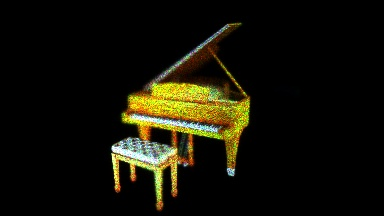
\includegraphics[width=\textwidth]{bcom_piano4k.jpg}
    \caption{Holograma \texttt{Piano4k} (imagem original).}
    \label{fig:bcom_piano4k}
\end{figure}


\section{Conclusões}
\label{sec::tecno-ferr:conclusao}

Após a seleção das tecnologias e materiais, conforme supra-mencionados, ir-se-á proceder no Capítulo \ref{ch::imp-test} ao delineamento da estratégia de investigação do projeto, a qual está intimamente ligada às escolhas apresentadas no presente Capítulo, entre elas a escolha da linguagem Python para transcrição do \textit{software} original de reconstrução de hologramas, o \ac{SDK} para realizar a codificação no formato JPEG2000 e os hologramas testados.

\clearpage{\thispagestyle{empty}\cleardoublepage}
\chapter{Etapas de Desenvolvimento e Implementação}
\label{chap:imp-test}

\section{Introdução}
\label{chap4:sec:intro}

\section{Reconstrução dos Hologramas}
\label{chap4:sec:...}

O projeto iniciou-se com uma pesquisa exaustiva sobre a ciência da holografia, a qual resultou no Estado da Arte resumido no Capítulo \ref{chap:estado-da-arte}.

Simultaneamente, foi efetuado um estudo das funções do \textit{software} desenvolvido no âmbito do projeto JPEG Pleno a fim de se poder fazer a respetiva transcrição para Python.

\begin{table}[!htbp]
    \centering
    \caption{Resumo da documentação da função \texttt{load\_hologram}.}
    \label{tab:load_hologram}
    \begin{tabular}{p{1cm} p{10cm}}
        \hline
        \multicolumn{2}{l}{\bfseries Nome da função}\\
         & \verb|load_hologram|\\
        \hline
        \multicolumn{2}{l}{\bfseries Protótipo original em MATLAB}\\
         & \mintinline[breaklines]{matlab}{function [hologram] = load_hologram(ampli_path, phase_path)}\\
        \hline
        \multicolumn{2}{l}{\bfseries Protótipo transcrito em Python}\\
         & \mintinline{python}{def load_hologram(ampli_path, phase_path)} \\
        \hline\multicolumn{2}{l}{\bfseries Descrição}\\
         & Esta função carrega um holograma da base de dados b<>com a partir dos seus ficheiros de amplitude e fase.\\
        \hline\multicolumn{2}{l}{\bfseries \textit{Inputs}}\\
         & \verb|ampli_path|: Diretório do ficheiro da imagem da amplitude (caminho relativo ou absoluto).\\
         & \verb|phase_path|: Diretório do ficheiro da imagem da fase (caminho relativo ou absoluto).\\
        \hline\multicolumn{2}{l}{\bfseries \textit{Output}}\\
         & Modulação complexa do holograma (3 canais: R-G-B).\\
        \hline
    \end{tabular}
\end{table}


\begin{table}[!htbp]
    \centering
    \caption{Resumo da documentação da função \texttt{propagate\_asm}.}
    \label{tab:propagate_asm}
    \begin{tabular}{p{1cm} p{10cm}}
        \hline
        \multicolumn{2}{l}{\bfseries Nome da função}\\
         & \verb|propagate_asm|\\
        \hline
        \multicolumn{2}{l}{\bfseries Protótipo original em MATLAB}\\
         & \mintinline[breaklines]{matlab}{function [v] = propagate_asm(u, pitch, wavelength, z)}\\
        \hline
        \multicolumn{2}{l}{\bfseries Protótipo transcrito em Python}\\
         & \mintinline[breaklines]{python}{def propagate_asm(u, pitch, wavelength, z)} \\
        \hline\multicolumn{2}{l}{\bfseries Descrição}\\
         & Esta função simula a propagação no plano complexo \verb|u| sobre a distância \verb|z| utilizando o \ac{ASM}.\\
        \hline\multicolumn{2}{l}{\bfseries \textit{Inputs}}\\
         & \verb|u|: Campo de onda de luz do plano de \textit{input} (um canal).\\
         & \verb|pitch|: Distância entre pixeis (em metros).\\
         & \verb|wavelength|: Comprimento de onda do canal de cor a propagar (em metros).\\
         & \verb|z|: Distância de propagação ao longo do eixo ótico (em metros).\\
        \hline\multicolumn{2}{l}{\bfseries \textit{Output}}\\
         & Campo de onda de luz no plano de destino (um canal).\\
        \hline
    \end{tabular}
\end{table}


\begin{table}[!htbp]
    \centering
    \caption{Resumo da documentação da função \texttt{reconst\_hologram}.}
    \label{tab:reconst_hologram}
    \begin{tabular}{p{1cm} p{10cm}}
        \hline
        \multicolumn{2}{l}{\bfseries Nome da função}\\
         & \verb|reconst_hologram|\\
        \hline
        \multicolumn{2}{l}{\bfseries Protótipo original em MATLAB}\\
         & \mintinline[breaklines]{matlab}{function [recons] = reconsHologram(hologram, pitch, wavelengths, z, pupilPos, pupilSize)
         }\\
        \hline
        \multicolumn{2}{l}{\bfseries Protótipo transcrito em Python}\\
         & \mintinline[breaklines]{python}{def reconst_hologram(hologram, pitch, wavelengths, z, pupil_pos=[0,0], pupil_size=None)} \\
        \hline\multicolumn{2}{l}{\bfseries Descrição}\\
         & Esta função reconstrói o holograma a uma distância \verb|z|, utilizando o \ac{ASM}. Permite o uso de uma janela para obter reconstruções de diferentes pontos de vista.\\
        \hline\multicolumn{2}{l}{\bfseries \textit{Inputs}}\\
         & \verb|hologram|: Holograma de modulação complexa (3 canais: R-G-B). \\
         & \verb|pitch|: Distância entre pixeis (em metros).\\
         & \verb|wavelengths|: Comprimentos de onda de luz (em metros, 3 canais: R-G-B).\\
         & \verb|z|: Distância de reconstrução (em metros).\\
         & \verb|pupilPos|: Posição da janela (em pixeis, canto superior direito).\\
         & \verb|pupilSize|: Tamanho da janela (em pixeis, altura $\times$ largura).\\
        \hline\multicolumn{2}{l}{\bfseries \textit{Output}}\\
         & Reconstrução numérica do holograma (3 canais: R-G-B).\\
        \hline
    \end{tabular}
\end{table}

% - Estudo holografia
% - estudo funções matlab
% transcrever funções para scripts em python
% comparar output entre funções de matlab e python para confirmar que os hologramas estão a ser reconstruidos corretamente
% desenvolver script para reconstruir o mesmo holograma de 16 vistas diferentes


\section{Compressão dos Hologramas Reconstruídos}
\lipsum[1]
% automatização de execução dos softwares
% estudar o uso de kdu
% implementar script que comprime com e sem transformada de cor, e com bitrates: [0.1, 0.3, 0.6, 1.0, 1.5, 2.0, 2.5, 3.0, 3.5, 4.0, 4.5, 5.0], e descomprime as reconstruções do holograma

\section{Determinação das Métricas de Compressão}
\lipsum[1]
% calcular o débito com a métrica PSNR entre o holograma original e a imagem comprimida
% estudar qual a melhor forma de guardar os débitos calculados
% implementar no script a escrita dos dados num ficheiro json
% a partir dos ficheiros json gerados, criar gráficos para apresentar os resultados com uso da biblioteca matplotlib.pyplot








\section{Conclusões}
\label{chap4:sec:concs}

\clearpage{\thispagestyle{empty}\cleardoublepage}
\chapter{Testes e Resultados}
% Os titulos dados aos capítulos são meros exemplos. Cada relatório deve adequar-se ao projeto desenvolvido.
\label{ch::test-result}

\section{Introdução}
\label{sec::test-result:intro}

TODO


\section{Resultados}
\label{sec::test-result:result}

TODO


\section{Conclusões}
\label{chap4:sec:concs}
\label{sec::estado-arte:concs}

TODO
\clearpage{\thispagestyle{empty}\cleardoublepage}
\chapter{Conclusões e Trabalho Futuro}
\label{chap:conc-trab-futuro}

\section{Conclusões Principais}
\label{sec:conc-princ}

Esta secção contém a resposta à questão: \\
\emph{Quais foram as conclusões princípais a que o(a) aluno(a) chegou no fim deste trabalho?}

\section{Trabalho Futuro}
\label{sec:trab-futuro}

Esta secção responde a questões como:\\
\emph{O que é que ficou por fazer, e porque?}\\
\emph{O que é que seria interessante fazer, mas não foi feito por não ser exatamente o objetivo deste trabalho?}\\
\emph{Em que outros casos ou situações ou cenários -- que não foram estudados no contexto deste projeto por não ser seu objetivo -- é que o trabalho aqui descrito pode ter aplicações interessantes e porque?}
\clearpage{\thispagestyle{empty}\cleardoublepage}

% SE EXISTIREM APENDICES, DESCOMENTAR O QUE ESTÁ EM BAIXO
% \appendix
% \include{apendice1}
% \clearpage{\pagestyle{empty}\cleardoublepage}
% \include{continuacao}
% \clearpage{\pagestyle{empty}\cleardoublepage}
% \include{apendice2}
% \clearpage{\pagestyle{empty}\cleardoublepage}
% \include{apendice3}
% \clearpage{\pagestyle{empty}\cleardoublepage}

\backmatter

\bibliographystyle{plain}
\nocite{*}
% \bibliography{bibliografia}

\end{document}